\documentclass[journal]{IEEEtran}

% ---------------------------------------------------------------
% Packages
% ---------------------------------------------------------------
\usepackage{cite}
\usepackage{amsmath,amssymb,amsfonts}
\usepackage{graphicx}
\usepackage{textcomp}
\usepackage{xcolor}
\usepackage{booktabs}
\usepackage{url}
\usepackage{hyperref}
\usepackage{float}
\usepackage{placeins}

\graphicspath{{figures_supplementary/}}

% Number every figure as S1, S2, ... so the labels match the citations
% used in the main manuscript.
\renewcommand{\thefigure}{S\arabic{figure}}

% Float spacing
\setlength{\textfloatsep}{8pt plus 2pt minus 4pt}
\setlength{\floatsep}{6pt plus 2pt minus 2pt}
\setlength{\intextsep}{8pt plus 2pt minus 2pt}

% ---------------------------------------------------------------
\begin{document}

\title{Supplementary Material\\
\large Evaluating Predictive Utility of Synthetic Liver Cirrhosis Data in IoMT: A Comparative Study of GAN, CTGAN, and TVAE with Consensus-Based Quality Filtering}

\author{\IEEEauthorblockN{Michael~Udousoro,~MSc~and~Mohammad~Farhan~Khan,~\IEEEmembership{PhD, Senior Lecturer}}
\IEEEauthorblockA{\textit{Department of Computer Science}\\
\textit{University of Roehampton}\\
London, United Kingdom}}

\maketitle

\section*{Overview}

This document contains ten supporting figures referenced in the main manuscript as Fig.~S1 to Fig.~S10. They fall into two groups.

Figures~S1 to~S5 give additional detail on the dataset and on the distributional behaviour of the three generative models: the correlation structure of the real cohort, the training curves of each model, and three complementary views of how closely the synthetic records match real patients.

Figures~S6 to~S10 present graphical views of the predictive results. Every quantity plotted in this second group also appears numerically in Tables~III and~IV of the main paper; the figures are provided for readers who prefer a visual comparison and are not the primary evidence for any claim.

All figures were produced by the pipeline described in Section~III of the main paper, run under fixed random seeds (Python, NumPy, and TensorFlow all seeded at 42). The code that generates them is available at \url{https://github.com/Michaeludousoro/liver-cirrhosis-synthetic-data}.

\FloatBarrier
\section*{Dataset and Generative Model Behaviour}

\begin{figure}[!t]
  \centering
  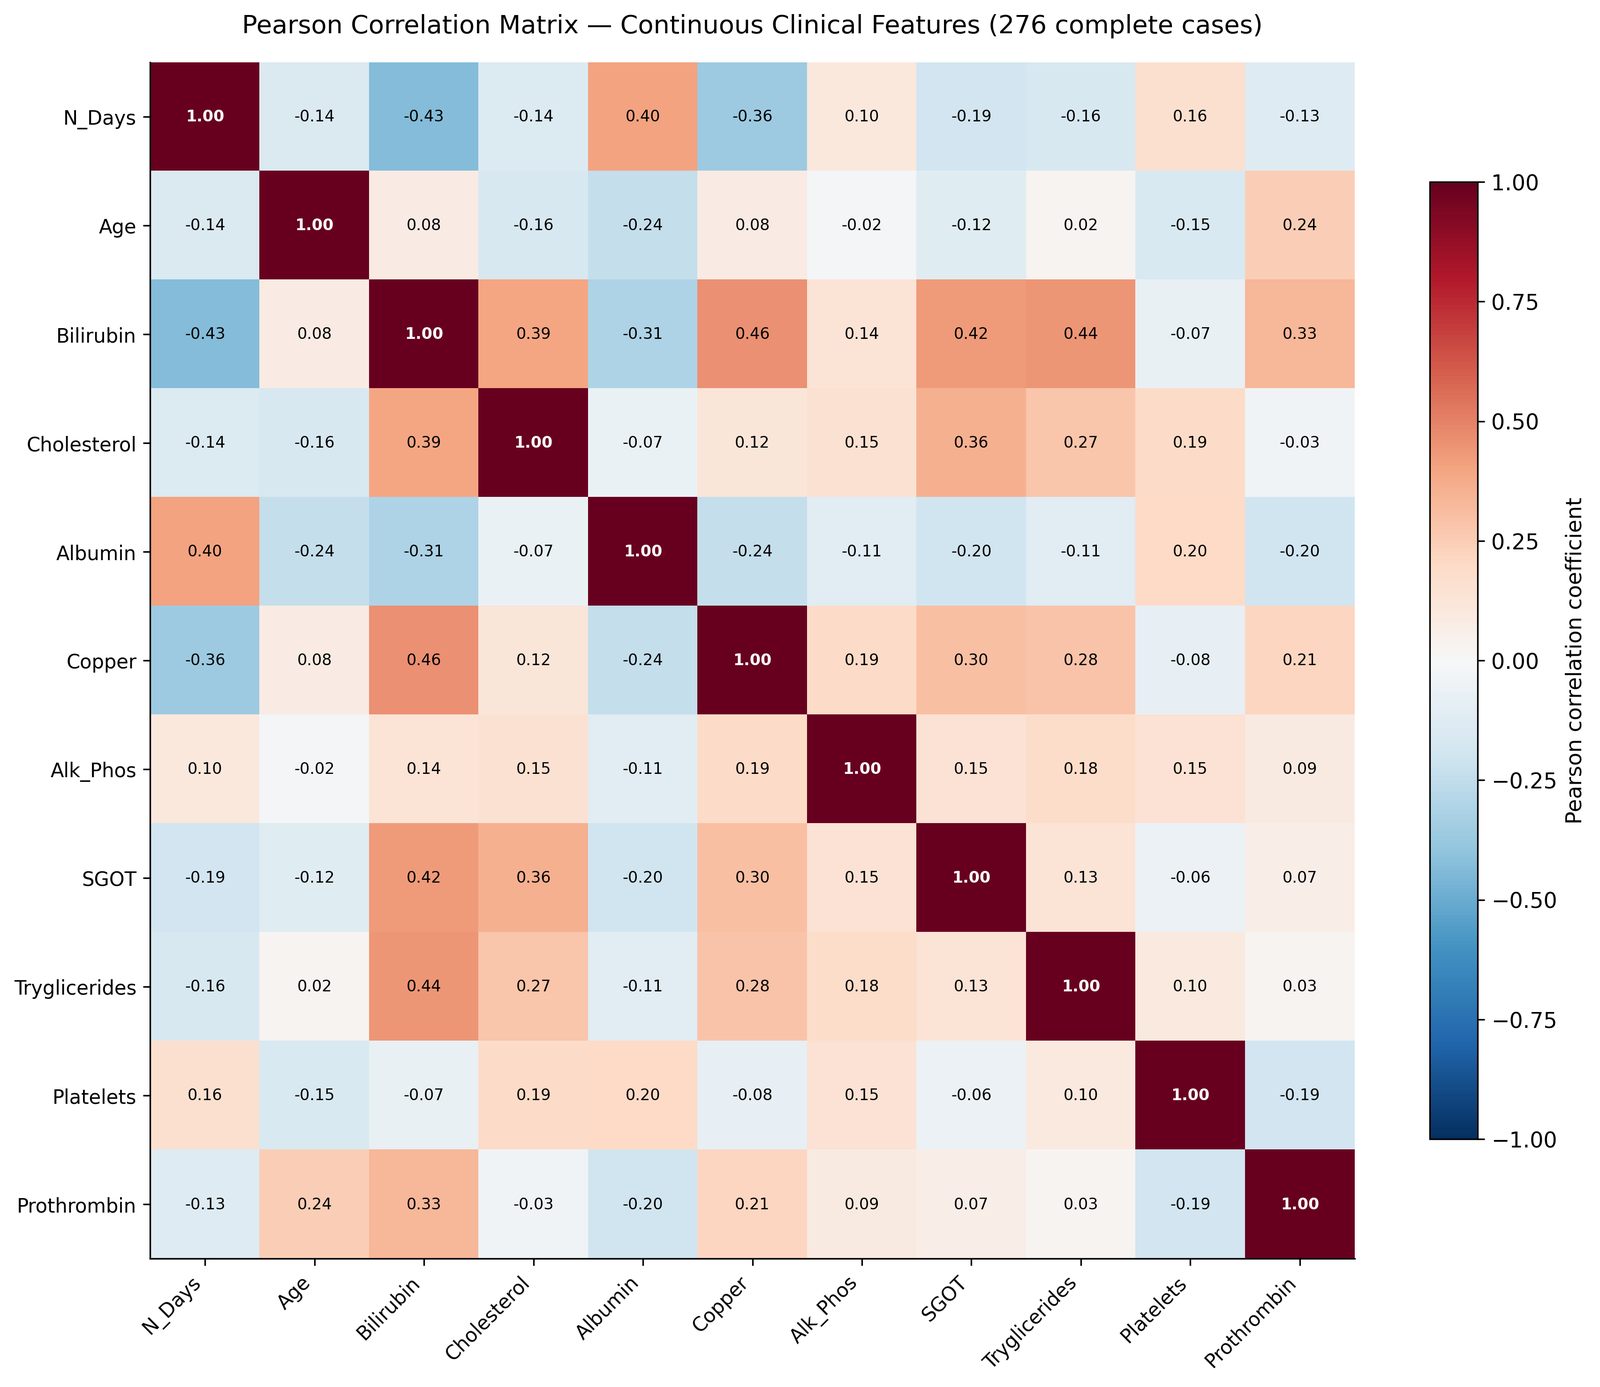
\includegraphics[width=\columnwidth]{figS01_correlation_matrix.png}
  \caption{Pearson correlation matrix across all 276 complete cases. Bilirubin shows strong positive correlations with Copper ($r = 0.46$), SGOT ($r = 0.42$), Cholesterol ($r = 0.39$), and Prothrombin ($r = 0.33$), reflecting the interlinked nature of hepatic synthetic and excretory function in PBC. N\_Days is negatively correlated with Bilirubin ($r = -0.43$) and Copper ($r = -0.36$), consistent with more severe biochemical profiles being associated with shorter survival.}
  \label{figS:corrmatrix}
\end{figure}

\begin{figure}[!t]
  \centering
  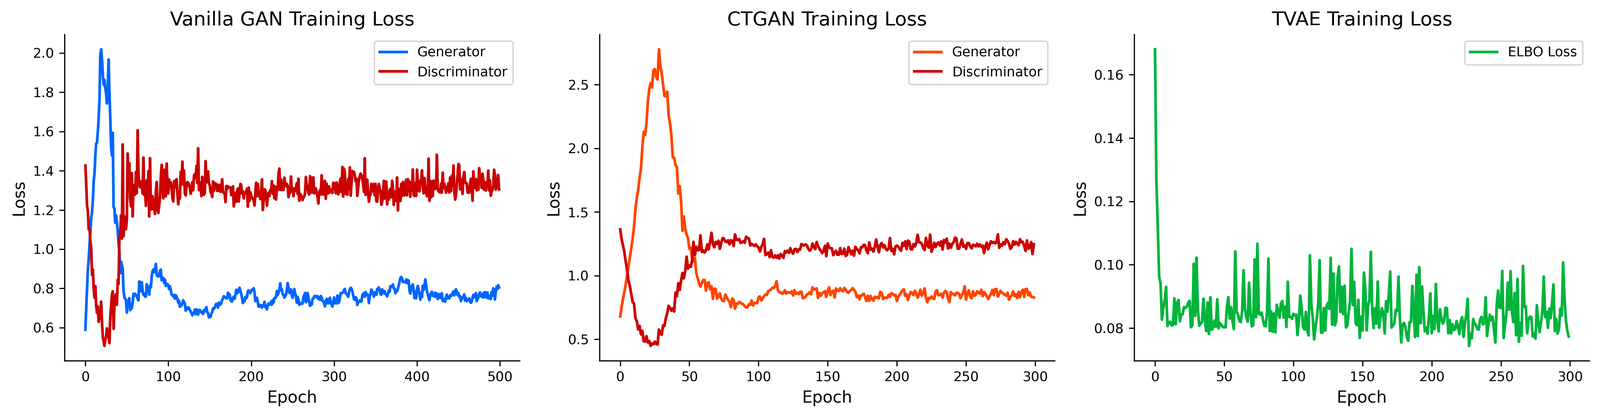
\includegraphics[width=\columnwidth]{figS02_training_losses.png}
  \caption{Training loss curves for all three generative models. Left: Vanilla GAN generator and discriminator losses over 500 epochs. Centre: conditional tabular GAN losses over 300 epochs. Right: TVAE total ELBO loss over 300 epochs. The adversarial losses settle without the sustained oscillation that indicates mode collapse, and the TVAE ELBO falls steeply before levelling off, so all three models reach convergence within their training budgets.}
  \label{figS:training}
\end{figure}

\begin{figure}[!t]
  \centering
  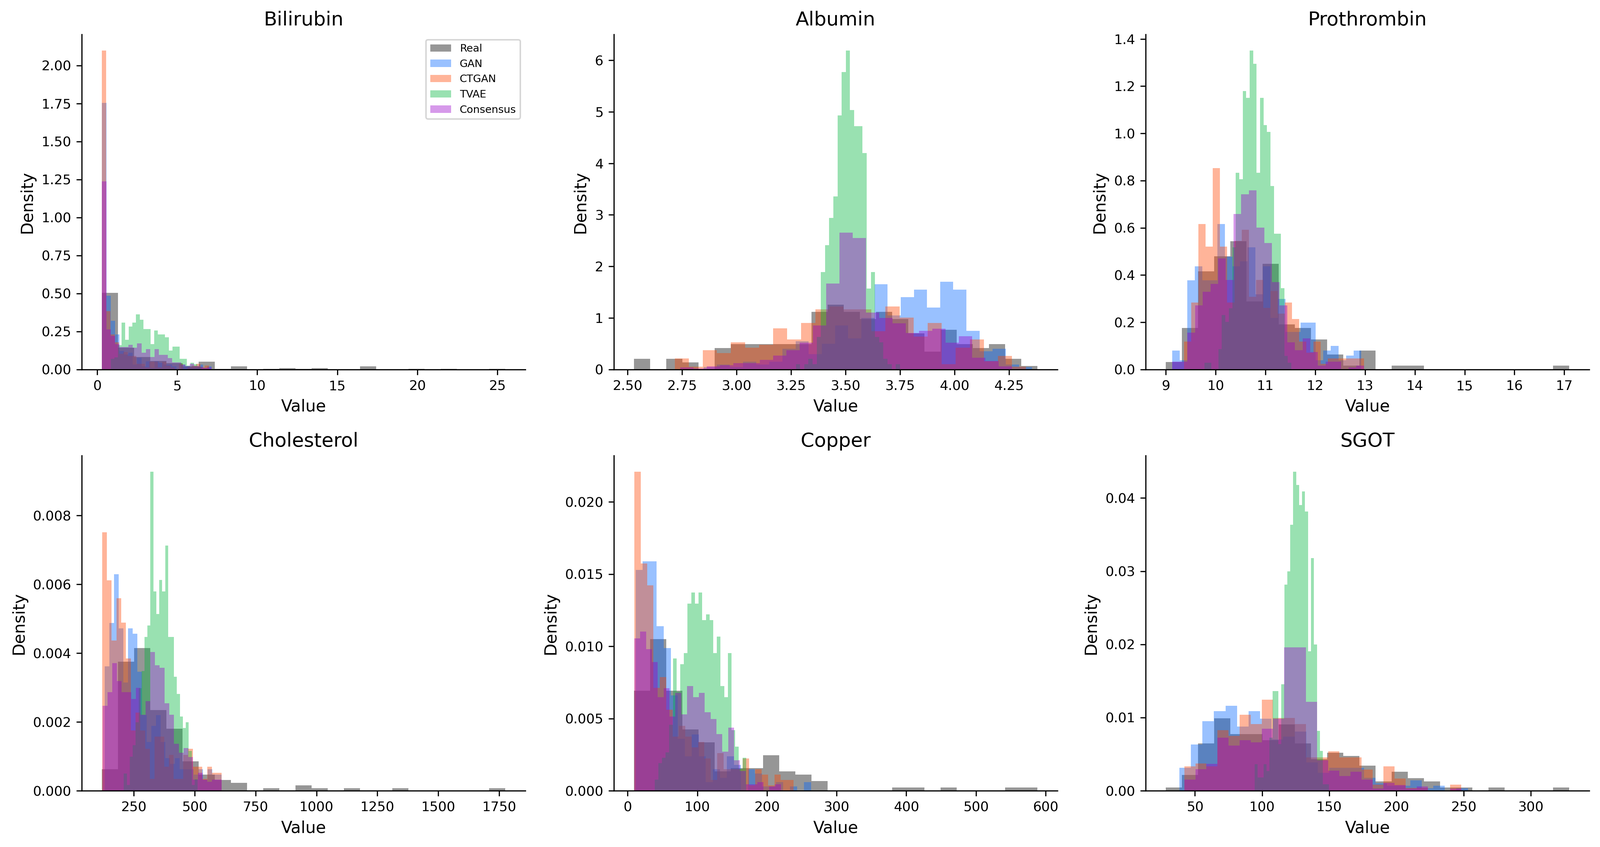
\includegraphics[width=\columnwidth]{figS03_distribution_comparison.png}
  \caption{Feature distribution comparison between real training data and all four synthetic datasets for six representative clinical variables: Bilirubin, Albumin, Prothrombin, Cholesterol, Copper, and SGOT. GAN and CTGAN reproduce Albumin and Prothrombin closely, while all methods diverge on the heavily right-skewed Bilirubin and Cholesterol features. The TVAE distribution for Bilirubin is shifted noticeably rightward relative to real patients.}
  \label{figS:distributions}
\end{figure}

\begin{figure}[!t]
  \centering
  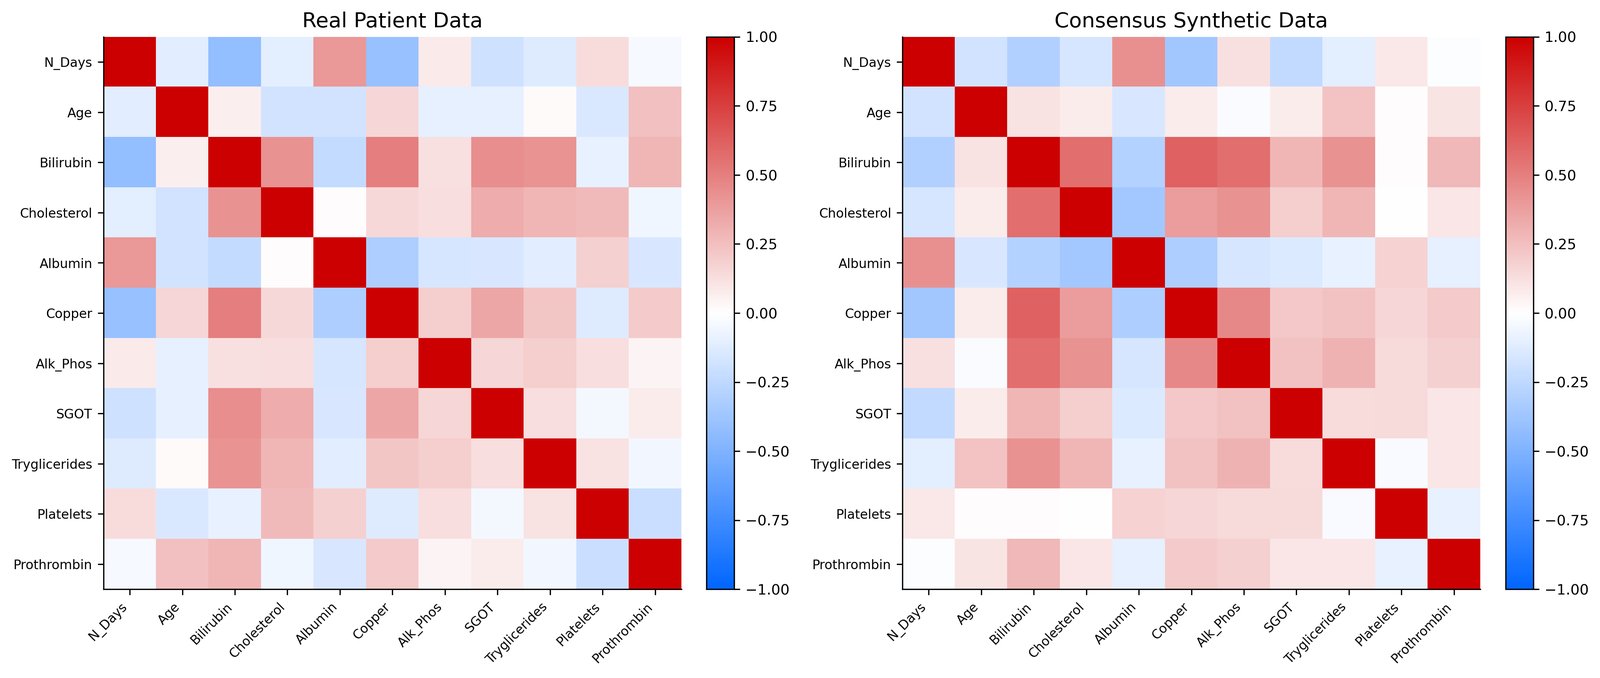
\includegraphics[width=\columnwidth]{figS04_correlation_heatmap.png}
  \caption{Pearson correlation structure of real patient data (left) compared with the equalised consensus synthetic set (right). The consensus set preserves the dominant clinical associations, including the positive Bilirubin-Copper relationship ($r = 0.46$ in real data) and the negative N\_Days-Bilirubin association ($r = -0.43$), although weaker correlations are attenuated.}
  \label{figS:corrcomparison}
\end{figure}

\begin{figure}[!t]
  \centering
  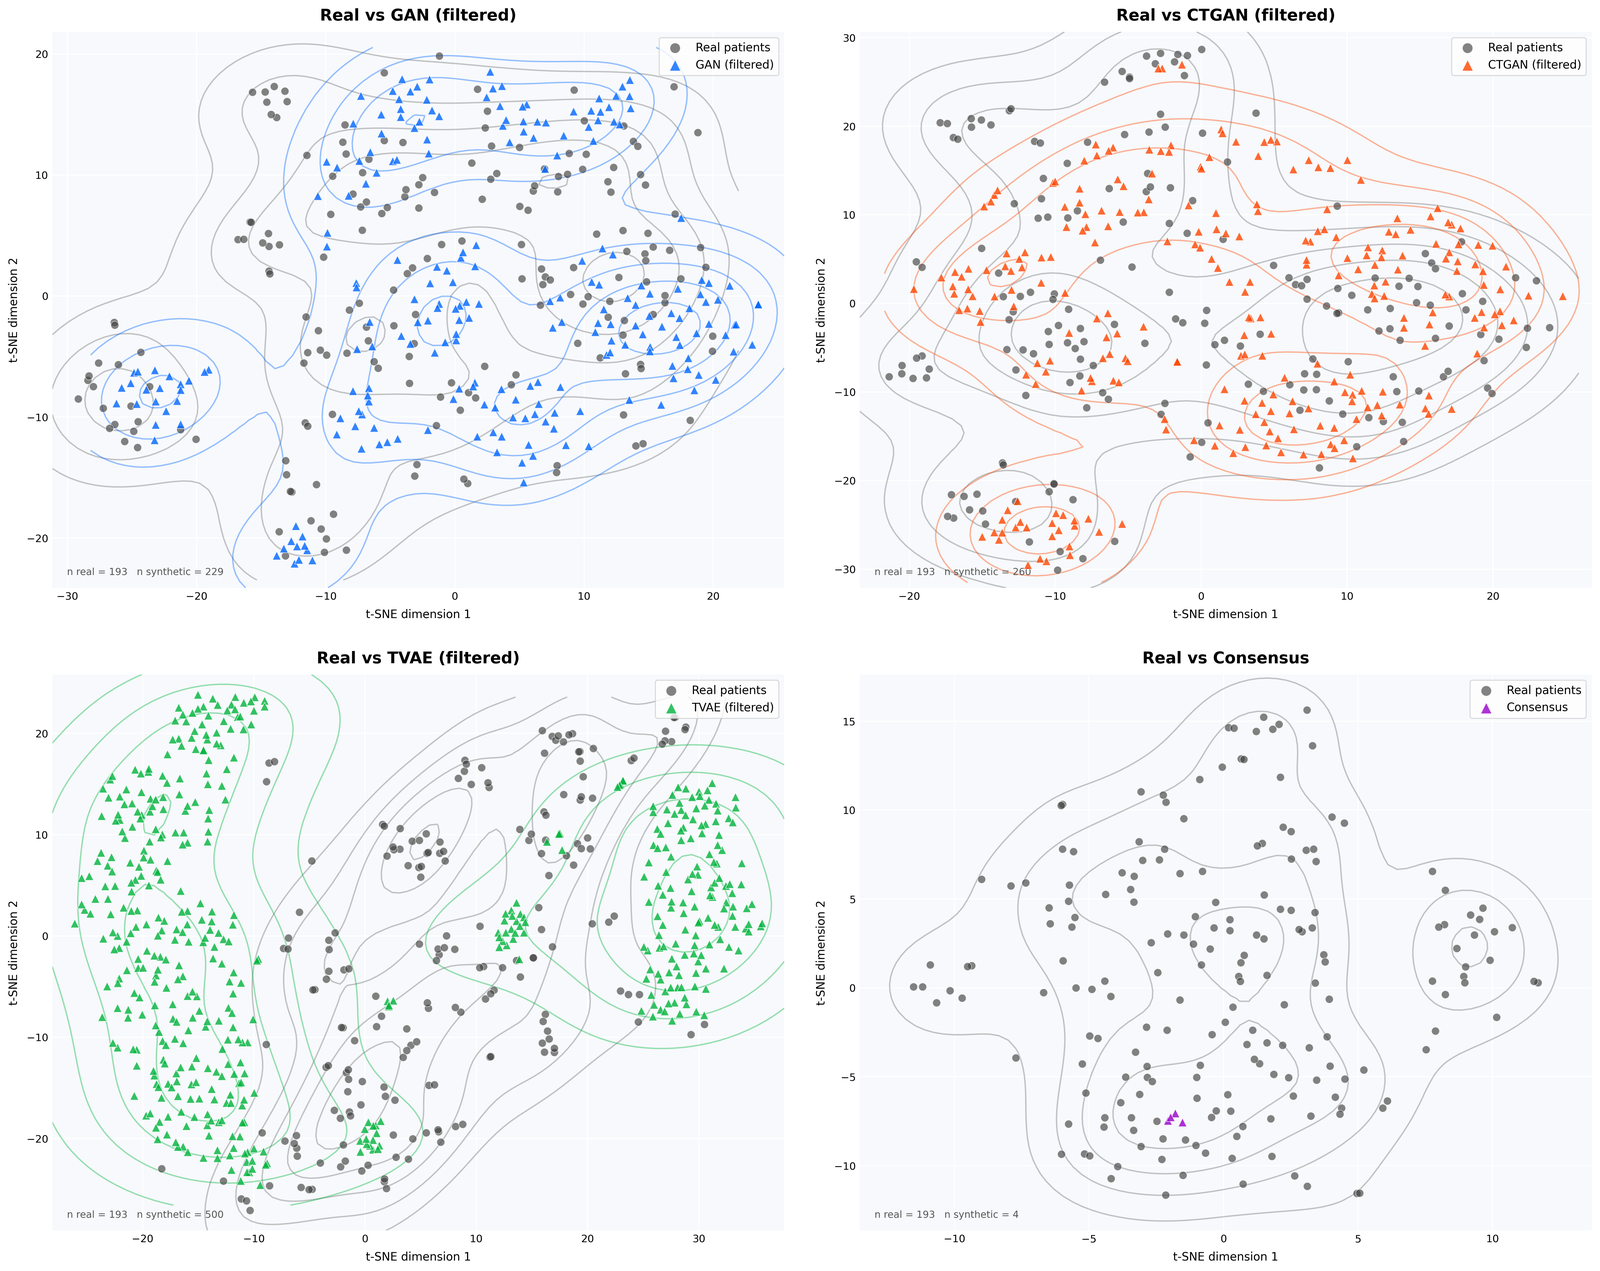
\includegraphics[width=\columnwidth]{figS05_tsne_projection.png}
  \caption{t-SNE two-dimensional projection of real patients and each synthetic method from the original 18-dimensional feature space. The filtered GAN and CTGAN sets overlap the real patient manifold. TVAE points spread more widely, with portions falling outside the real patient density contours. The consensus set concentrates in the central high-density region, which is consistent with its elevated near-duplicate rate reported in Table~II of the main paper.}
  \label{figS:tsne}
\end{figure}

\FloatBarrier
\section*{Graphical Views of the Predictive Results}

\begin{figure}[!t]
  \centering
  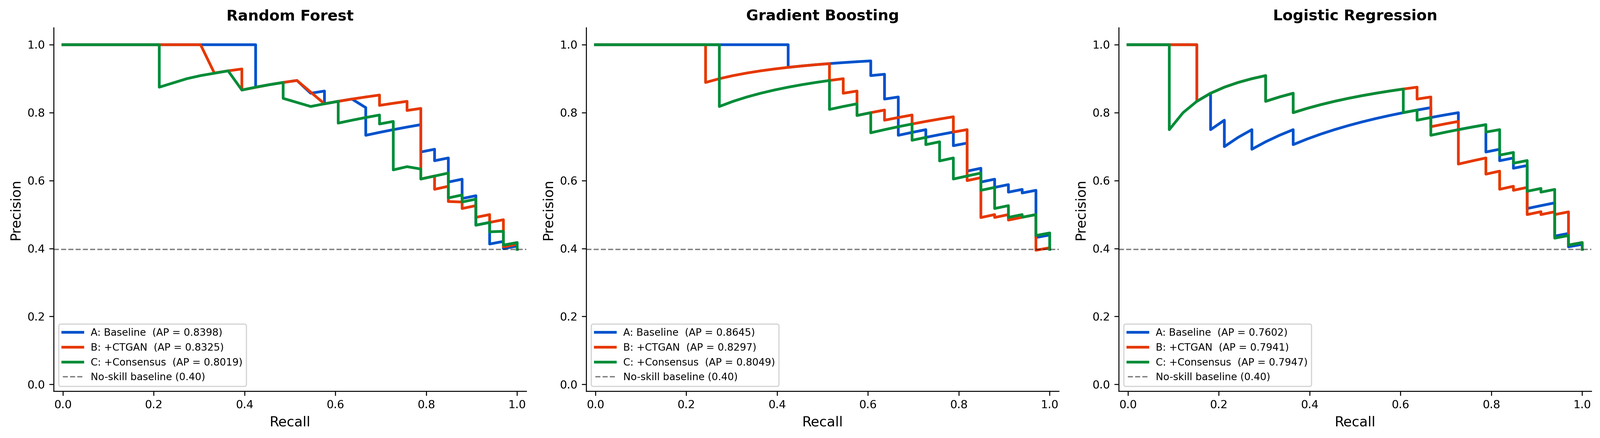
\includegraphics[width=\columnwidth]{figS06_pr_curves.png}
  \caption{Precision-Recall curves by classifier and training scenario on the 83-patient real held-out test set. PR curves are informative for this cohort given its class imbalance (78 deceased versus 115 survivors in the training set). All classifiers hold precision above 0.7 across a wide recall range.}
  \label{figS:prcurves}
\end{figure}

\begin{figure}[!t]
  \centering
  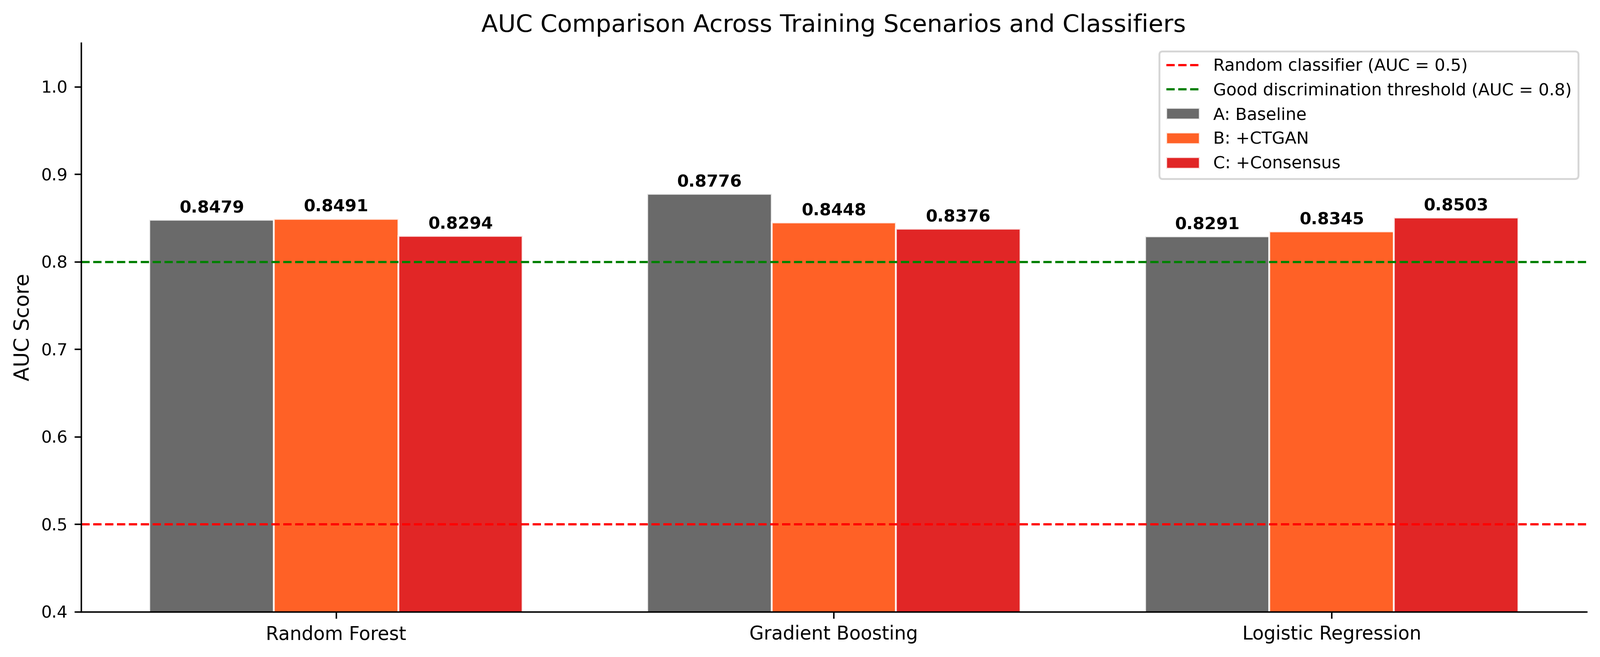
\includegraphics[width=\columnwidth]{figS07_auc_comparison.png}
  \caption{AUC scores across all three classifiers and training scenarios A through D. The green dashed reference line marks AUC~$= 0.8$ and the red dashed line marks AUC~$= 0.5$. Every scenario and classifier combination clears 0.8, confirming that no augmentation strategy degrades discrimination below a clinically useful threshold. Gradient Boosting under Scenario~A achieves the highest AUC at 0.878.}
  \label{figS:auc}
\end{figure}

\begin{figure}[!t]
  \centering
  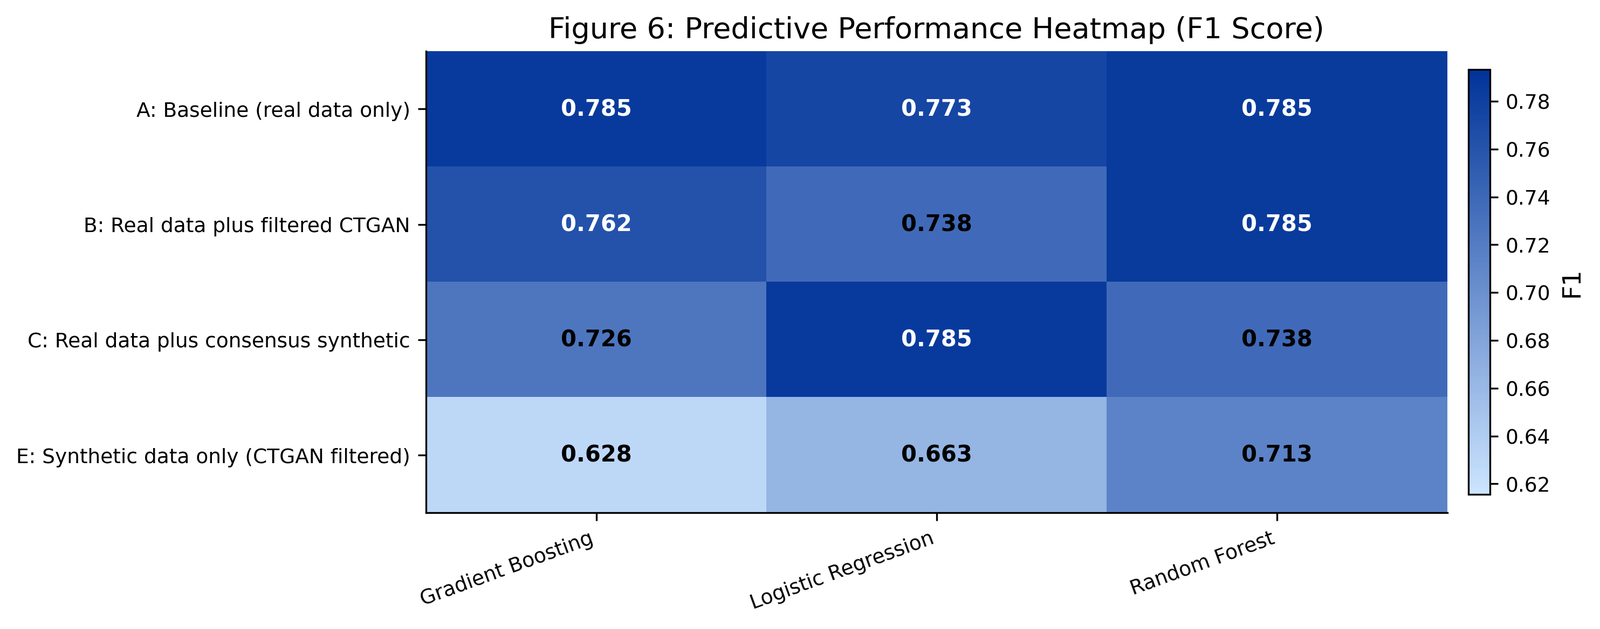
\includegraphics[width=\columnwidth]{figS08_performance_heatmap.png}
  \caption{F1-score heatmap across training scenarios for all three classifiers; darker shading indicates higher F1. Gradient Boosting under Scenario~D achieves the highest F1 at 0.809. Under Scenario~C, Gradient Boosting falls to 0.726 and Random Forest to 0.738, while Logistic Regression rises to 0.785, illustrating that consensus augmentation does not move all classifiers in the same direction.}
  \label{figS:heatmap}
\end{figure}

\begin{figure}[!t]
  \centering
  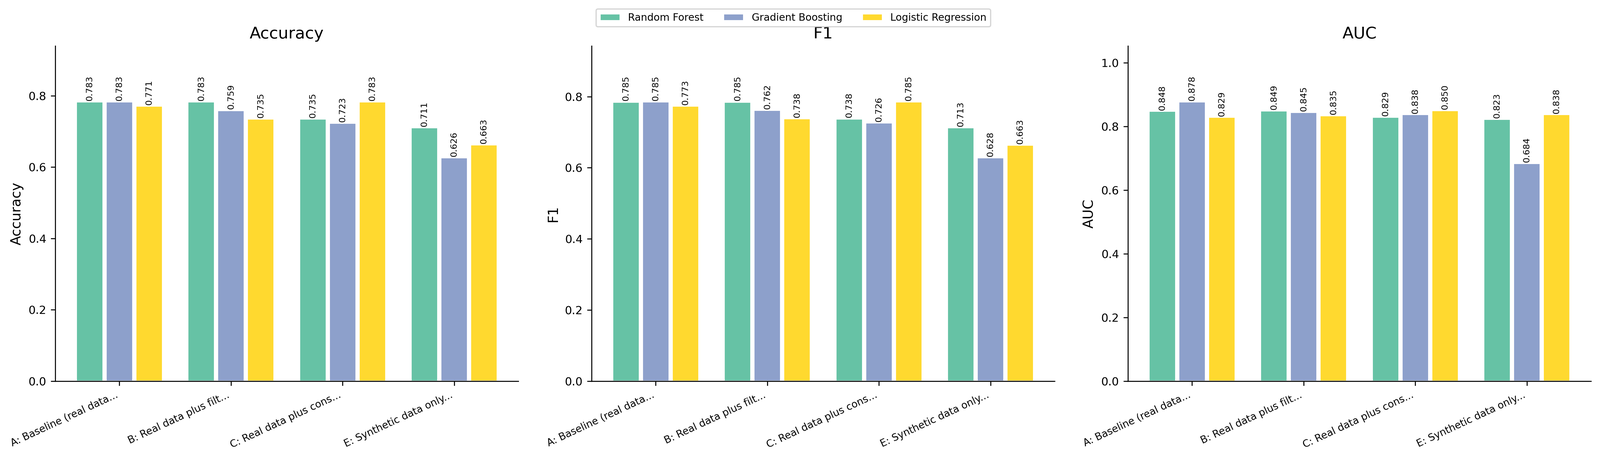
\includegraphics[width=\columnwidth]{figS09_model_comparison.png}
  \caption{Grouped bar chart comparing accuracy, F1, and AUC across all training scenarios and classifiers. No augmentation scenario uniformly outperforms the real-data baseline across all classifiers and metrics.}
  \label{figS:modelcomp}
\end{figure}

\begin{figure}[!t]
  \centering
  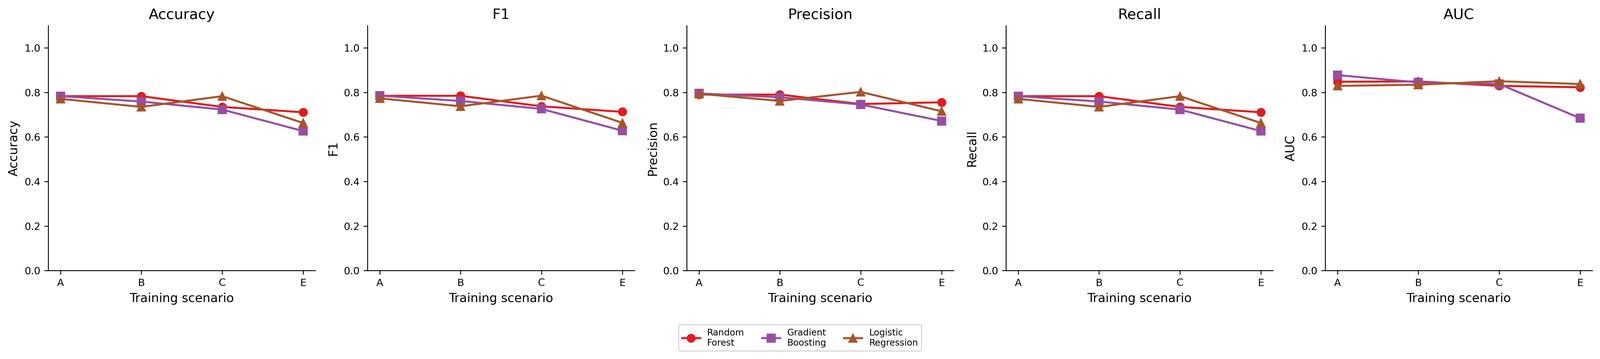
\includegraphics[width=\columnwidth]{figS10_all_metrics.png}
  \caption{All five evaluation metrics (Accuracy, F1, Precision, Recall, AUC) across training scenarios for each classifier. Trajectories are generally flat or slightly declining from Scenario~A through Scenarios~B and~C, with Scenario~D producing a modest accuracy gain for Gradient Boosting.}
  \label{figS:allmetrics}
\end{figure}

\FloatBarrier

\end{document}
